\chapter{Superconducting solenoid system for COMET experiment}
~~~~~~COMET phase-I experiment is aiming to measure the background and search the $\mu \rightarrow e$ conversion with the sensitivity of 10$^{-14}$.
Its superconducting magnet system consists of pion capture solenoid, muon transport solenoid and detector solenoid.
In phase-II experiment, nowadays' 90 degree bent transport solenoid will be extended to 180 degree curved solenoid, and another spectrometer solenoid will be added.
 
\section{Superconducting magnet system}
~~~~~~Superconducting magnet system plays a key role in pion capture, muon transport and signal tracking.
In the case of COMET phase-I experiment, the 8 GeV proton with high intensity is injected into superconducting magnet and hits the target to produce pion, then these backward pions are captured by pion capture solenoid, which provides 5 Tesla magnetic field at peak.
Muons with low momentum from the decay of captured pions are transported to stopping target by the muon transport solenoid with 3 Tesla.
Because the high momentum muon and the other particles will cause the background on detector, the muon transport solenoid is designed with 90 degree curve to throw out these particles.
After the muon captured by stopping target, the emitted electron from stopping target will be bent by detector solenoid which provides 1 Tesla magnetic field and tracked in cylindrical drift chamber (CDC).

The schematic layout of COMET superconducting solenoid is given in figure~\ref{solenoid}.
Pion capture solenoid consists of CS0, CS1, MS1, MS2 and TS1a-TS1f superconducting coils.
Meanwhile, muon transport solenoid includes TS2, TS3 and BS coils, and detector solenoid has 12 DS coils.
\begin{figure}[H]
 \centering
 \includegraphics[scale=0.45]{chapter2/fig/solenoid.pdf}
 \caption{Schematic layout of superconducting magnet system for COMET phase-I experiment.}
 \label{solenoid}
\end{figure}

 \section{Pion capture solenoid}
~~~~~~Pion capture solenoid is most critical magnet for capturing the pions from production target with a large solid angle.
Considering the valleys of magnetic field causes the trapping of charged particle, the magnetic field distribution must be smooth.
The details of the magnetic field of pion capture solenoid is shown in table~\ref{magfldcs}.
\begin{table}[H]
 \centering
 \begin{tabular}{ccccccc} \hline \hline
  Coils & B$_z$ & Inner radius & Outer radius & Length & Current & Current density \\
   & [T] & [mm] & [mm] & [mm] & [A] & [A/mm$^2$] \\ \hline
  CS0 & 4.0 & 662 & 806 & 175 & 2700 & 33.75 \\
  CS1 & 5.0 & 662 & 806 & 1350 & 2700 & 33.75 \\
  MS1 & 4.0 & 662 & 742 & 1425 & 2700 & 33.75 \\
  MS2 & 3.0 & 662 & 774 & 700 & 2700 & 33.75 \\
  TS1a & 3.0 & 250 & 266 & 200 & 2700 & 33.75 \\
  TS1b & 3.0 & 250 & 298 & 240 & 2581 & 32.26 \\
  TS1c & 3.0 & 250 & 314 & 200 & 2700 & 33.75 \\
  TS1d & 3.0 & 250 & 314 & 200 & 2619 & 32.74 \\
  TS1e & 3.0 & 250 & 298 & 200 & 2538 & 31.73 \\
  TS1f & 3.0 & 400 & 496 & 350 & 2916 & 36.45 \\ \hline \hline
 \end{tabular}
 \caption{Details of coils for pion capture solenoid.}
 \label{magfldcs}
\end{table}
All of the superconducting coils in pion capture solenoid is connected together with the same current provided by one power supply.
Furthermore, conduction cooling is employed in whole COMET superconducting magnet system due to the tritium production under high radiation environment by reaction of $^3$He(n,p)$^3$H.
Also the direct cooling needs helium vessel and the coils must be enlarged, the more radiation and stored energy deposits in larger coils.
From all aspect, the conduction cooling is the best choice for COMET superconducting magnet system.
Aluminum-stabilized conductors is used in all the coils for reducing the heat load and preventing the over heat of coils after quench.

\subsection{Coils structure}
~~~~~~To reduce the energy deposition in coils, superconducting wires are all merged with 5N aluminum (0.1\% Ni) due to its low density.
The reason why 
0.1\% nickel is mixed to enhance the mechanical property of conductor.
\begin{figure}[H]
 \centering
 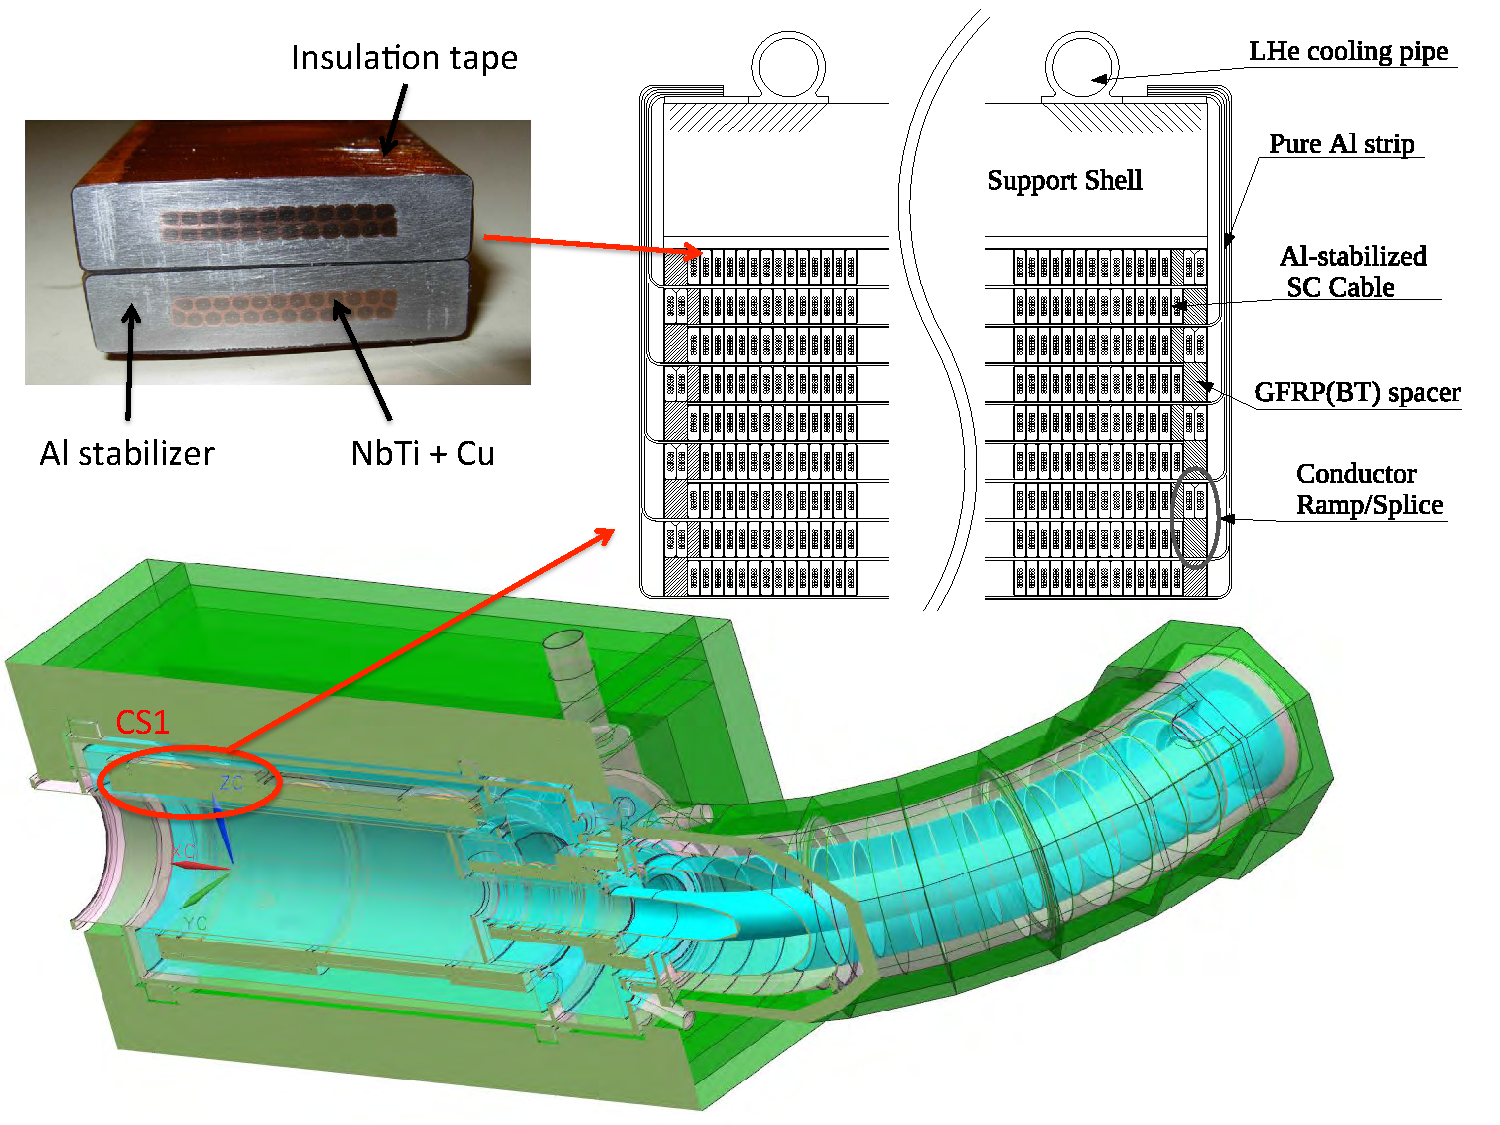
\includegraphics[scale=0.45]{chapter2/fig/coil.pdf}
 \caption{\it Coil and conductor structure of CS1.}
 \label{cssrtu}
\end{figure}

The aluminum-stabilized conductor with the size of 15.0 $\times$ 4.7 mm$^2$ is wound with two layers of insulation tape, which is made of polyimide film covered by boron free glass with BT and epoxy resin.
Here, The reason why BT and epoxy resin is used because it has good mechanical property under the high radiation.
In addition, the insulated conductor is impregnated by the BT and epoxy resin mixed with silica filler during the coils winding.

The coil structure of CS1 and detail of design parameters are shown in figure~\ref{cssrtu} and table~\ref{desip} respectively.
There are 9 layers superconducting coils totally, and each layer is cooled by inserting 1 mm thick pure aluminum strip with RRR of 2000.
Each aluminum strip is installed between two conductor layers, and connected to the liquid helium cooling pipe.
Support shell with 5 cm thick is located on the top of superconducting coils to suppress the deformation of coils.
\begin{table}[H]
 \centering
 \begin{tabular}{ll} \hline \hline
  Item & Value \\ \hline
  Conductor & Aluminum stabilized SC cable \\
   & Al:Cu:NbTi = 7.3:0.9:1 \\
  Cable dimensions & 15.0 $\times$ 4.7 mm$^2$ (without insulation) \\
   & 15.3 $\times$ 5.0 mm$^2$ (with insulation) \\
  Cable insulation & Polyimide film/Boron-free glass cloth \\
   & /BT-epoxy prepreg \\
  Magnet length & $\sim$ 6 m \\
  Number of coils & 10 \\
  Operation current & 2700 A \\
  Max. field on conductor & 5.5 T (T$_{cs}$ = 6.5 K) \\
  Stored energy & 47 MJ \\
  Coil layer & 9 (CS0+CS1), 5 (MS1), 7 (MS2), \\
   & 1$\sim$6 (TSa$\sim$TS1f) \\
  Quench protection & active quench back heater \\ \hline \hline
 \end{tabular}
 \caption{Details of design parameters for capture solenoid magnet.}
 \label{desip}
\end{table}

\subsection{Production target}
~~~~~~Production target is to make amounts of pions in the capture solenoid.
Phase-I is going to use the IG-43 graphite target rod with length of 60 cm, radius of 2 cm and density of 1.82 g/cm$^3$.
3.2 kW proton beam will deposit a heat load of approximately 100 W in the graphite target.
The temperature of target grows up to 190$^{\circ}$C at peak when 100 W energy is deposited in target.
A target support system accurately locates the target within the solenoid inner shield.

To achieve more pion production in COMET phase-II experiment, the target will be changed to pure tungsten rod with length of 16 cm and radius of 0.3 cm after the implementation of phase-I.
In addition, due to 56 kW proton beam power, phase-II target must be cooled on low temperature.
The proton beam also has to be fitted to a gaussian beam with 0.2 cm radius.

\subsection{Radiation shield}
~~~~~~A radiation shield is installed inside the CS and MS coils to protect superconducting coils from radiation.
This radiation shield has to be designed for both phase-I and phase-II experiment due to the high residual radiation.
The neutron came from production target directly is about 3$\times$10$^{12}$ n/cm$^2$/sec in COMET phase-II experiment, which corresponds to 10$^{24}$ n/m$^2$.
Both NbTi superconducting cable and stabilizers degrade if they are irradiated by neutrons with this order.
Therefore, due to a small radius of capture solenoid, a powerful radiation shield is needed to stop or decrease the radiation in short distance.
The most ideal radiation shield is made of pure tungsten with density of 19.25 g/cm$^3$.

However, to reduce the costs, a new composited radiation shield is designed and the details will be described in next chapter.

\subsection{Quench protection system}
~~~~~~Quench is caused by a hot spot in superconducting magnet.
When a hot spot quenches, temperature will rise suddenly, and propagate to all magnet.
Superconducting magnets has a risk of burn-out at temperature of quench.

Because the current becomes the joule heat after quench, decreasing the current quickly can suppress the temperature rise after quench.
There are two ways to speed up the current decay.
As shown in figure~\ref{dump}, one is to use the dump resistor in superconducting magnet circuit.
Once the quench is detected, the power supply will be turned off and current will flow towards to the dump resistor.
One quench protection diode is a switch for the quench protection circuit.
It is connected with superconducting wire and cooled to 4.2 K during operation.
The time constant is written as
\begin{equation}
 \tau = \frac{L}{R_{dump}}
\end{equation}
where $L$ is the inductance of magnets and $R_{dump}$ is the resistance of dump resistor respectively.
Higher resistance of dump resistor makes current decay quicker.
In the case of the pion capture solenoid, it is covered by the aluminum stabilizer.
Once quench is occurred, the current will flow into the aluminum stabilizer and copper matrix.
The current must decay more quickly due to the self resistance of stabilizer and matrix.
The time constant is written as
\begin{equation}
 \tau = \frac{L}{R_{dump} + R_{self}}
\end{equation}

Another way is to make the superconducting magnet quench to increase the self resistance by external heater.
It needs external power supply to heat the heater.
\begin{figure}[H]
 \begin{subfigure}{0.3\textwidth}
 \centering
 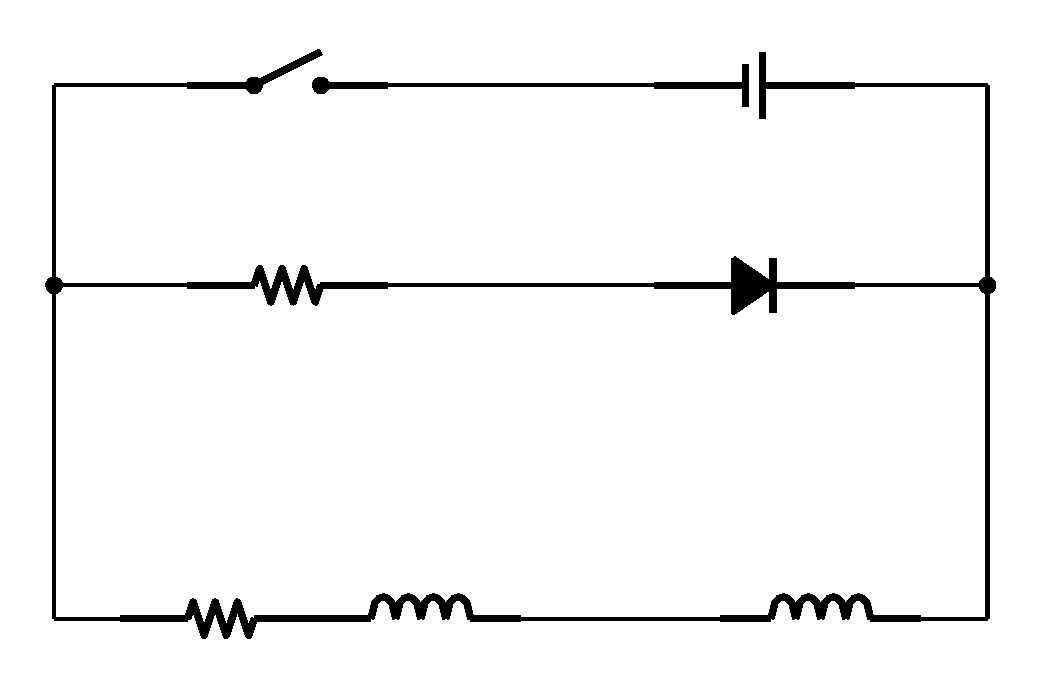
\includegraphics[scale=0.4]{chapter2/fig/dump.pdf}
 \end{subfigure}
 \hspace{0.2\textwidth}
 \begin{subfigure}{0.3\textwidth}
 \centering
 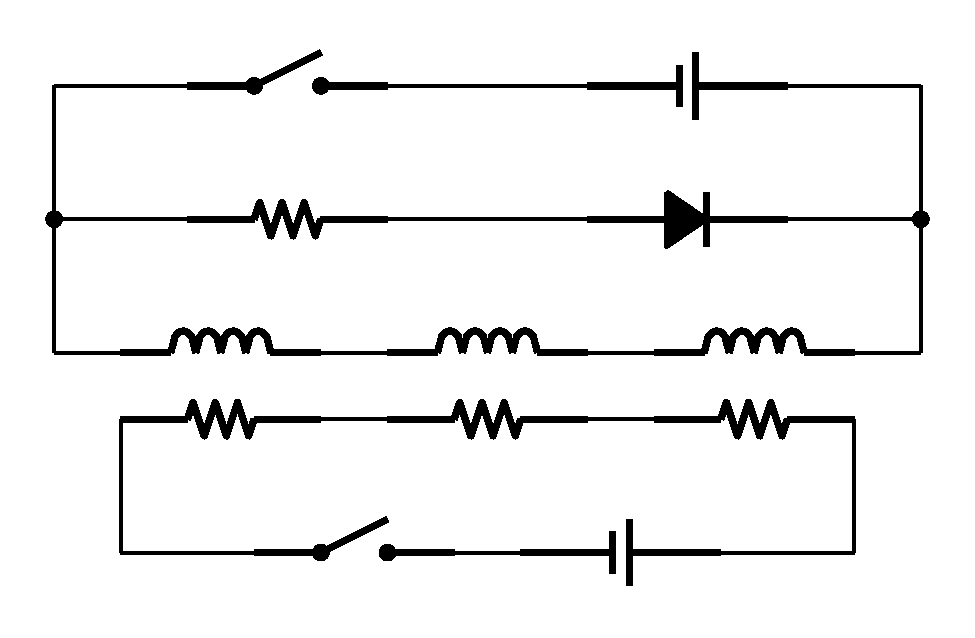
\includegraphics[scale=0.4]{chapter2/fig/heater.pdf}
 \end{subfigure}
 \caption{Schematics of quench protection circuit.}
 \label{dump}
\end{figure}

The quench protection system for pion capture solenoid is shown in figure~\ref{capture}.
All superconducting magnets in pion capture solenoid are connected together.
The power supply for capture solenoid is 2700 A, and 4 reserve trim power supplies and dump resistors are to reduce the current for TS1b, TS1d, TS1e and TS1f.
A dump resistor for capture solenoid is 0.185 $\Omega$, supposed the power supply is 500 V.
Once quench is occurred in one of the superconducting magnet of pion capture solenoid, the power supply will be turned off, and quench back heater will heat the all magnets.
Total resistivity of pion capture solenoid increases after heated, thus, the current will decay to zero in 1 min.
\begin{figure}[H]
 \centering
 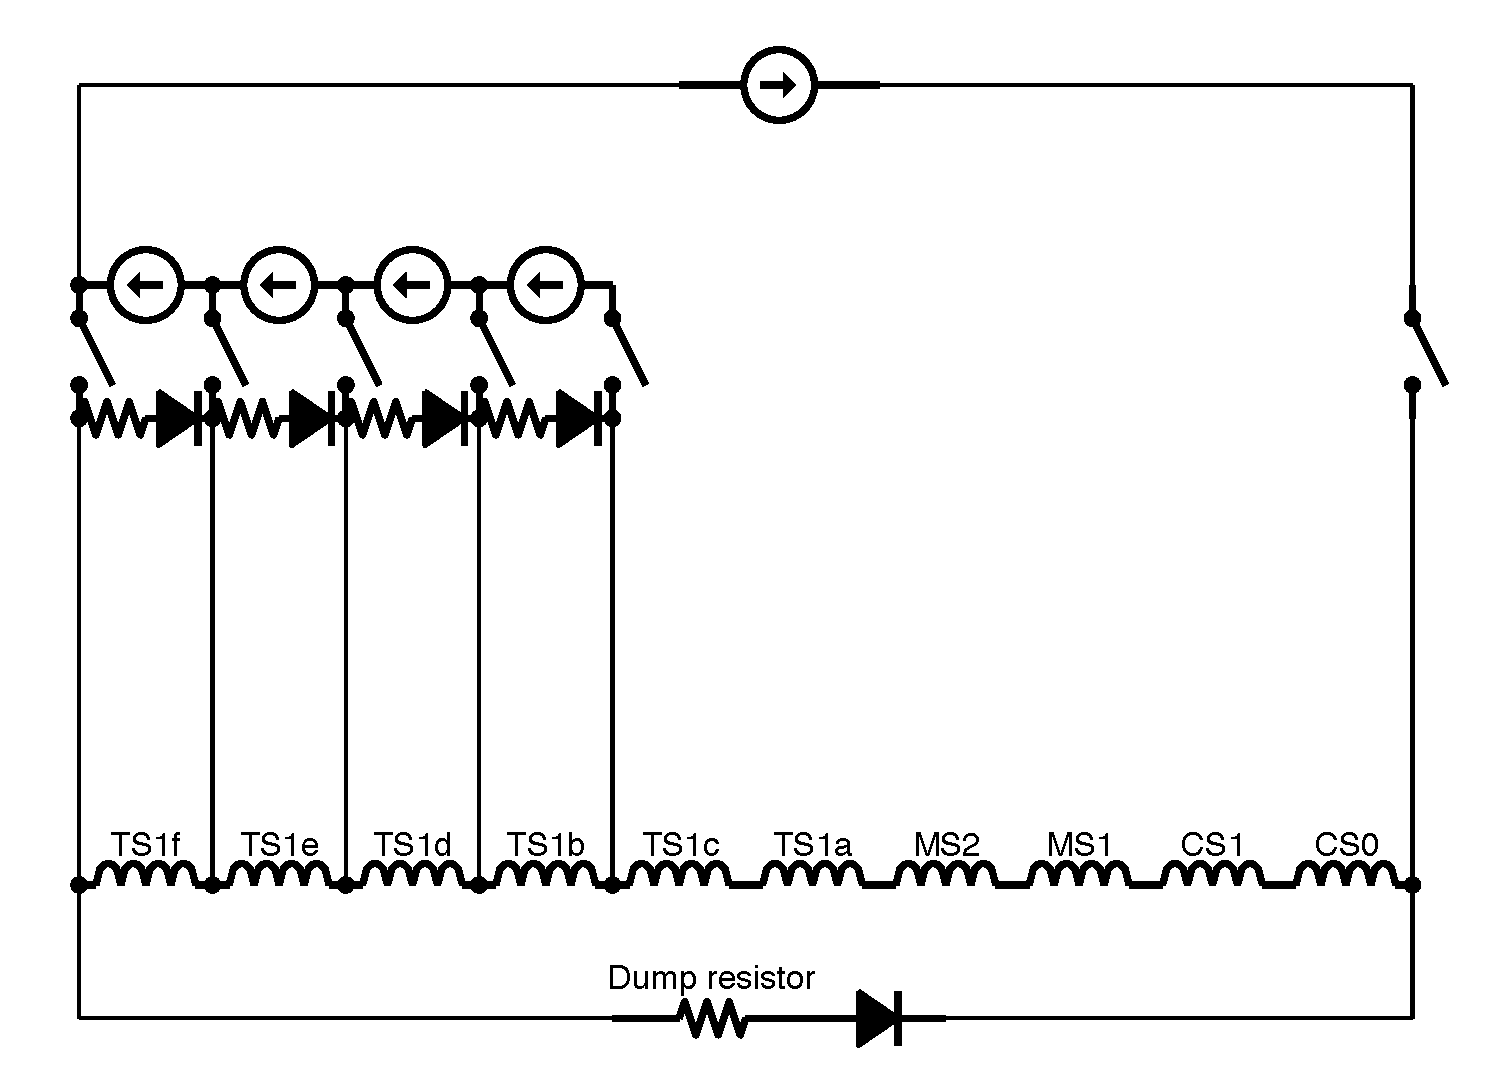
\includegraphics[scale=0.4]{chapter2/fig/capture.pdf}
 \caption{Schematics of quench protection system for pion capture solenoid.}
 \label{capture}
\end{figure}

 \section{Muon transport solenoid}
~~~~~~Muons are transported to the stopping target through the muon transport solenoid, which consists of curved superconducting magnets.
The muon transport solenoid must be designed to select the muons with low momentum and eliminate muons with high momentum ($p_{\mu^-} \textgreater$ 75 MeV/c), in addition, it also must be long enough for the pion decay.
Due to the beam dispersion in muon transport solenoid, the selection of charged particle depends on their momentum.
The magnitude of drift is given by
\begin{equation}
 D = \frac{1}{qB}(\frac{s}{R})\frac{p_L^2 + p_T^2/2}{p_L} = \frac{1}{qB}(\frac{s}{R})\frac{p}{2}(cos\theta + \frac{1}{cos\theta})
\end{equation}
where $q$ is the electric charge of particle, $B$ is the magnetic field, $s$ and $R$ are the path length and the radius of curvature of solenoid respectively.
$s/R$ is the bending angle, $p_L$ and $p_T$ [GeV/c] are longitudinal and transverse momnetum.
To keep the center of the helical trajectories of muons in the bending plane, a compensating dipole field parallel to the drift direction is applied, which is given by
\begin{equation}
 B_{comp} = \frac{1}{qR} \frac{p_0}{2} (cos\theta_0 + \frac{1}{cos\theta_0})
\end{equation}

The muon transport solenoid consists of 16 coils without stabilizer and a dipole coil with 0.056 Tesla compensating field is attached on the outer surface of each solenoid.
Details of each coil and design parameters are listed in table~\ref{tscoil} and \ref{designts}.
\begin{table}[H]
 \centering
 \begin{tabular}{cccccccc} \hline \hline
  Coil & B$_z$ & B$_y$ & Length & Inner radius & Outer radius & Current & Current density \\
   & [T] & [T] & [mm] & [mm] & [mm] & [A] & [A/mm$^2$] \\ \hline
  TS2a & 3 & NA & 255 & 234 & 249 & 210 & 72 \\
  TS2-1 & 3 & 0.06 & 205 & 234 & 264 & 210 & 95 \\
  TS2-2$\sim$15 & 3 & 0.06 & 205 & 234 & 272 & 210 & 95 \\
  TS2-16 & 3 & 0.06 & 205 & 234 & 254 & 210 & 94 \\
  TS3 & 3 & NA & 600 & 400 & 437 & 190 & 85.5 \\ \hline \hline
 \end{tabular}
 \caption{Coils parameters for muon transport solenoid.}
 \label{tscoil}
\end{table}
\begin{table}[H]
 \centering
 \begin{tabular}{ll} \hline \hline
  Item & Value \\ \hline
  Conductor & NbTi/Cu wire \\
   & Cu:NbTi = 6:1 \\
  Cable dimensions (solenoid) & $\phi$ 1.5 mm (without insulation) \\
   & $\phi$ 1.56 mm (with insulation) \\
  Cable dimensions (dipole) & $\phi$ 1.2 mm (without insulation) \\
   & $\phi$ 1.3 mm (with insulation) \\
  Cable insulation & Polyimide-imide enamel (AIW), \\
   & PVF (TS2-15, TS3) \\
  Magnet length & $\sim$ 6 m \\
  Curvature radius & 3 m \\
  Number of solenoid coils & 18 \\
  Number of dipole coils & 16 pairs \\
  Operation current & 210 A (solenoid) \\
   & 165 A (dipole) \\
  Field on axis & $\sim$ 3 T (solenoid) \\
   & $\sim$ 0.056 T (dipole) \\
  Stored energy & 5.6 MJ \\
  Total inductance & 254 H \\
  Refrigeration & conduction from forced flow 2-phase \\
   & LHe piping (7-10 g/sec) \\
  Quench protection & semi-active quench back heater \\ \hline \hline
 \end{tabular}
 \caption{Design parameters of transport solenoid.}
 \label{designts}
\end{table}


\section{Detector solenoid}
~~~~~~The detector solenoid consists of 14 DS coils and 5 BS collimator coils with 1 and 1.57 Tesla magnetic field respectively.
The superconducting wires of BS and DS have diameter of 1.26 mm with copper ratio of 4.2, and RRR of copper is higher than 60.
Superconducting cable is insulated by PVF with 30 $\mu$m thick.
The stored energy of DS and BS are about 4.45 MJ and 0.166 MJ respectively.
Inductance of these two solenoids are 240 H and 13.8 H.
The detector solenoid is cooled by GM refrigerators independently.
%\begin{table}[H]
% \centering
% \begin{tabular}{cccccccc} \hline \hline
%  Coil & B$_x$ & Length & Inner radius & Outer radius & Location & Current & Current density \\
%   & [T] & [mm] & [mm] & [mm] & [mm] & [A] & [A/mm$^2$] \\ \hline
%  BS1 & 1.57 & 300 & 230 & 241.1 & 10382.39 & 155 & 111 \\
%  BS2 & 1.57 & 150 & 230 & 245.5 & 10657.39 & 155 & 111 \\
%  BS3 & 1.57 & 240 & 310 & 320 & 10902.39 & 155 & 111 \\
%  BS4 & 1.57 & 180 & 310 & 320 & 11162.39 & 155 & 111 \\
%  BS5 & 1.57 & 180 & 310 & 320 & 11422.39 & 155 & 111 \\
%  DS1 & 1 & 170 & 1070 & 1078 & 11397.39 & 191 & 131 \\
%  DS2 & 1 & 170 & 1070 & 1078 & 11607.39 & 191 & 131 \\
%  DS3 & 1 & 170 & 1070 & 1078 & 11817.39 & 191 & 131 \\
%  DS4 & 1 & 170 & 1070 & 1078 & 12027.39 & 191 & 131 \\
%  DS5 & 1 & 170 & 1070 & 1078 & 12237.39 & 191 & 131 \\
%  DS6 & 1 & 170 & 1070 & 1078 & 12447.39 & 191 & 131 \\
%  DS7 & 1 & 170 & 1070 & 1078 & 12657.39 & 191 & 131 \\
%  DS8 & 1 & 170 & 1070 & 1078 & 12867.39 & 191 & 131 \\
%  DS9 & 1 & 170 & 1070 & 1078 & 13077.39 & 191 & 131 \\
%  DS10 & 1 & 170 & 1070 & 1078 & 13287.39 & 191 & 131 \\
%  DS11 & 1 & 170 & 1070 & 1078 & 13497.39 & 191 & 131 \\
%  DS12 & 1 & 170 & 1070 & 1078 & 13707.39 & 191 & 131 \\
%  DS13 & 1 & 170 & 1070 & 1078 & 13917.39 & 191 & 131 \\
%  DS14 & 1 & 170 & 1070 & 1078 & 14127.39 & 191 & 131 \\ \hline \hline
% \end{tabular}
% \caption{Dtails of coil for the collimator and detector solenoids.}
% \label{dsbs}
%\end{table}


